\documentclass{fisatproject}
\title{Website Design Ranking Using ML}
\team{Adhyaksh Guhan \\ Anet Eliza Johny\\ Dharwish Raj \\ Joel J Padayattil}
\author{Dharwish Raj}
\begin{document}
\maketitle

\makecert

\newpage
%\thispagestyle{plain}
\pagenumbering{roman}
\setcounter{page}{1}
\newgeometry{top=4cm,bottom=0.1cm}
\renewcommand\abstractname{ABSTRACT}
\begin{abstract}
\vspace{5cm}
Lorem ipsum dolor sit amet, consectetur adipiscing elit. Morbi urna mauris, sagittis sit amet aliquet ut, facilisis et nibh. Praesent turpis tortor, dignissim ut interdum eu, porttitor ut orci. Curabitur laoreet malesuada fermentum. In posuere, purus eu pulvinar luctus, eros urna tempor magna, eu tincidunt erat eros nec turpis. Vestibulum at semper lacus. Nullam tristique lacus vel nibh porta a vehicula tellus volutpat. Pellentesque cursus ullamcorper ante, ut eleifend nisl aliquam id. Nulla porta ornare fermentum. Aliquam id magna sed erat malesuada viverra. Donec non mauris eros, nec egestas ligula. Suspendisse eu tempor ligula. Aliquam egestas nulla vel augue iaculis iaculis nec in risus. Pellentesque habitant morbi tristique senectus et netus et malesuada fames ac turpis egestas. Praesent malesuada fringilla sapien a faucibus.
\end{abstract}


\newpage
%\thispagestyle{plain}
\renewcommand\abstractname{ACKNOWLEDGMENT}
\begin{abstract}
\vspace{5cm}
Your Acknowledgement Goes Here
\vspace{1cm}
\begin{flushright}
Student 1
\end{flushright}
\end{abstract}
\newpage

\restoregeometry
\tableofcontents
\newpage

\cleardoublepage
\addcontentsline{toc}{chapter}{\listfigurename}
\listoffigures
\newpage

\cleardoublepage
\addcontentsline{toc}{chapter}{\listtablename}
\listoftables
\newpage
\pagestyle{fancy}


\chapter{INTRODUCTION}
\pagenumbering{arabic}
\setcounter{page}{1}
\renewcommand{\baselinestretch}{1.50}
\section{Overview}
The mathematical roots of the idea of fractals have been traced through a formal path of published works, starting in the 17th century with notions of recursion, then moving through increasingly rigorous mathematical treatment of the concept to the study of continuous but not differentiable functions in the 19th century, and on to the coining of the word fractal in the 20th century with a subsequent burgeoning of interest in fractals and computer-based modelling in the 21st century.
\begin{figure}[h!]
\begin{center}
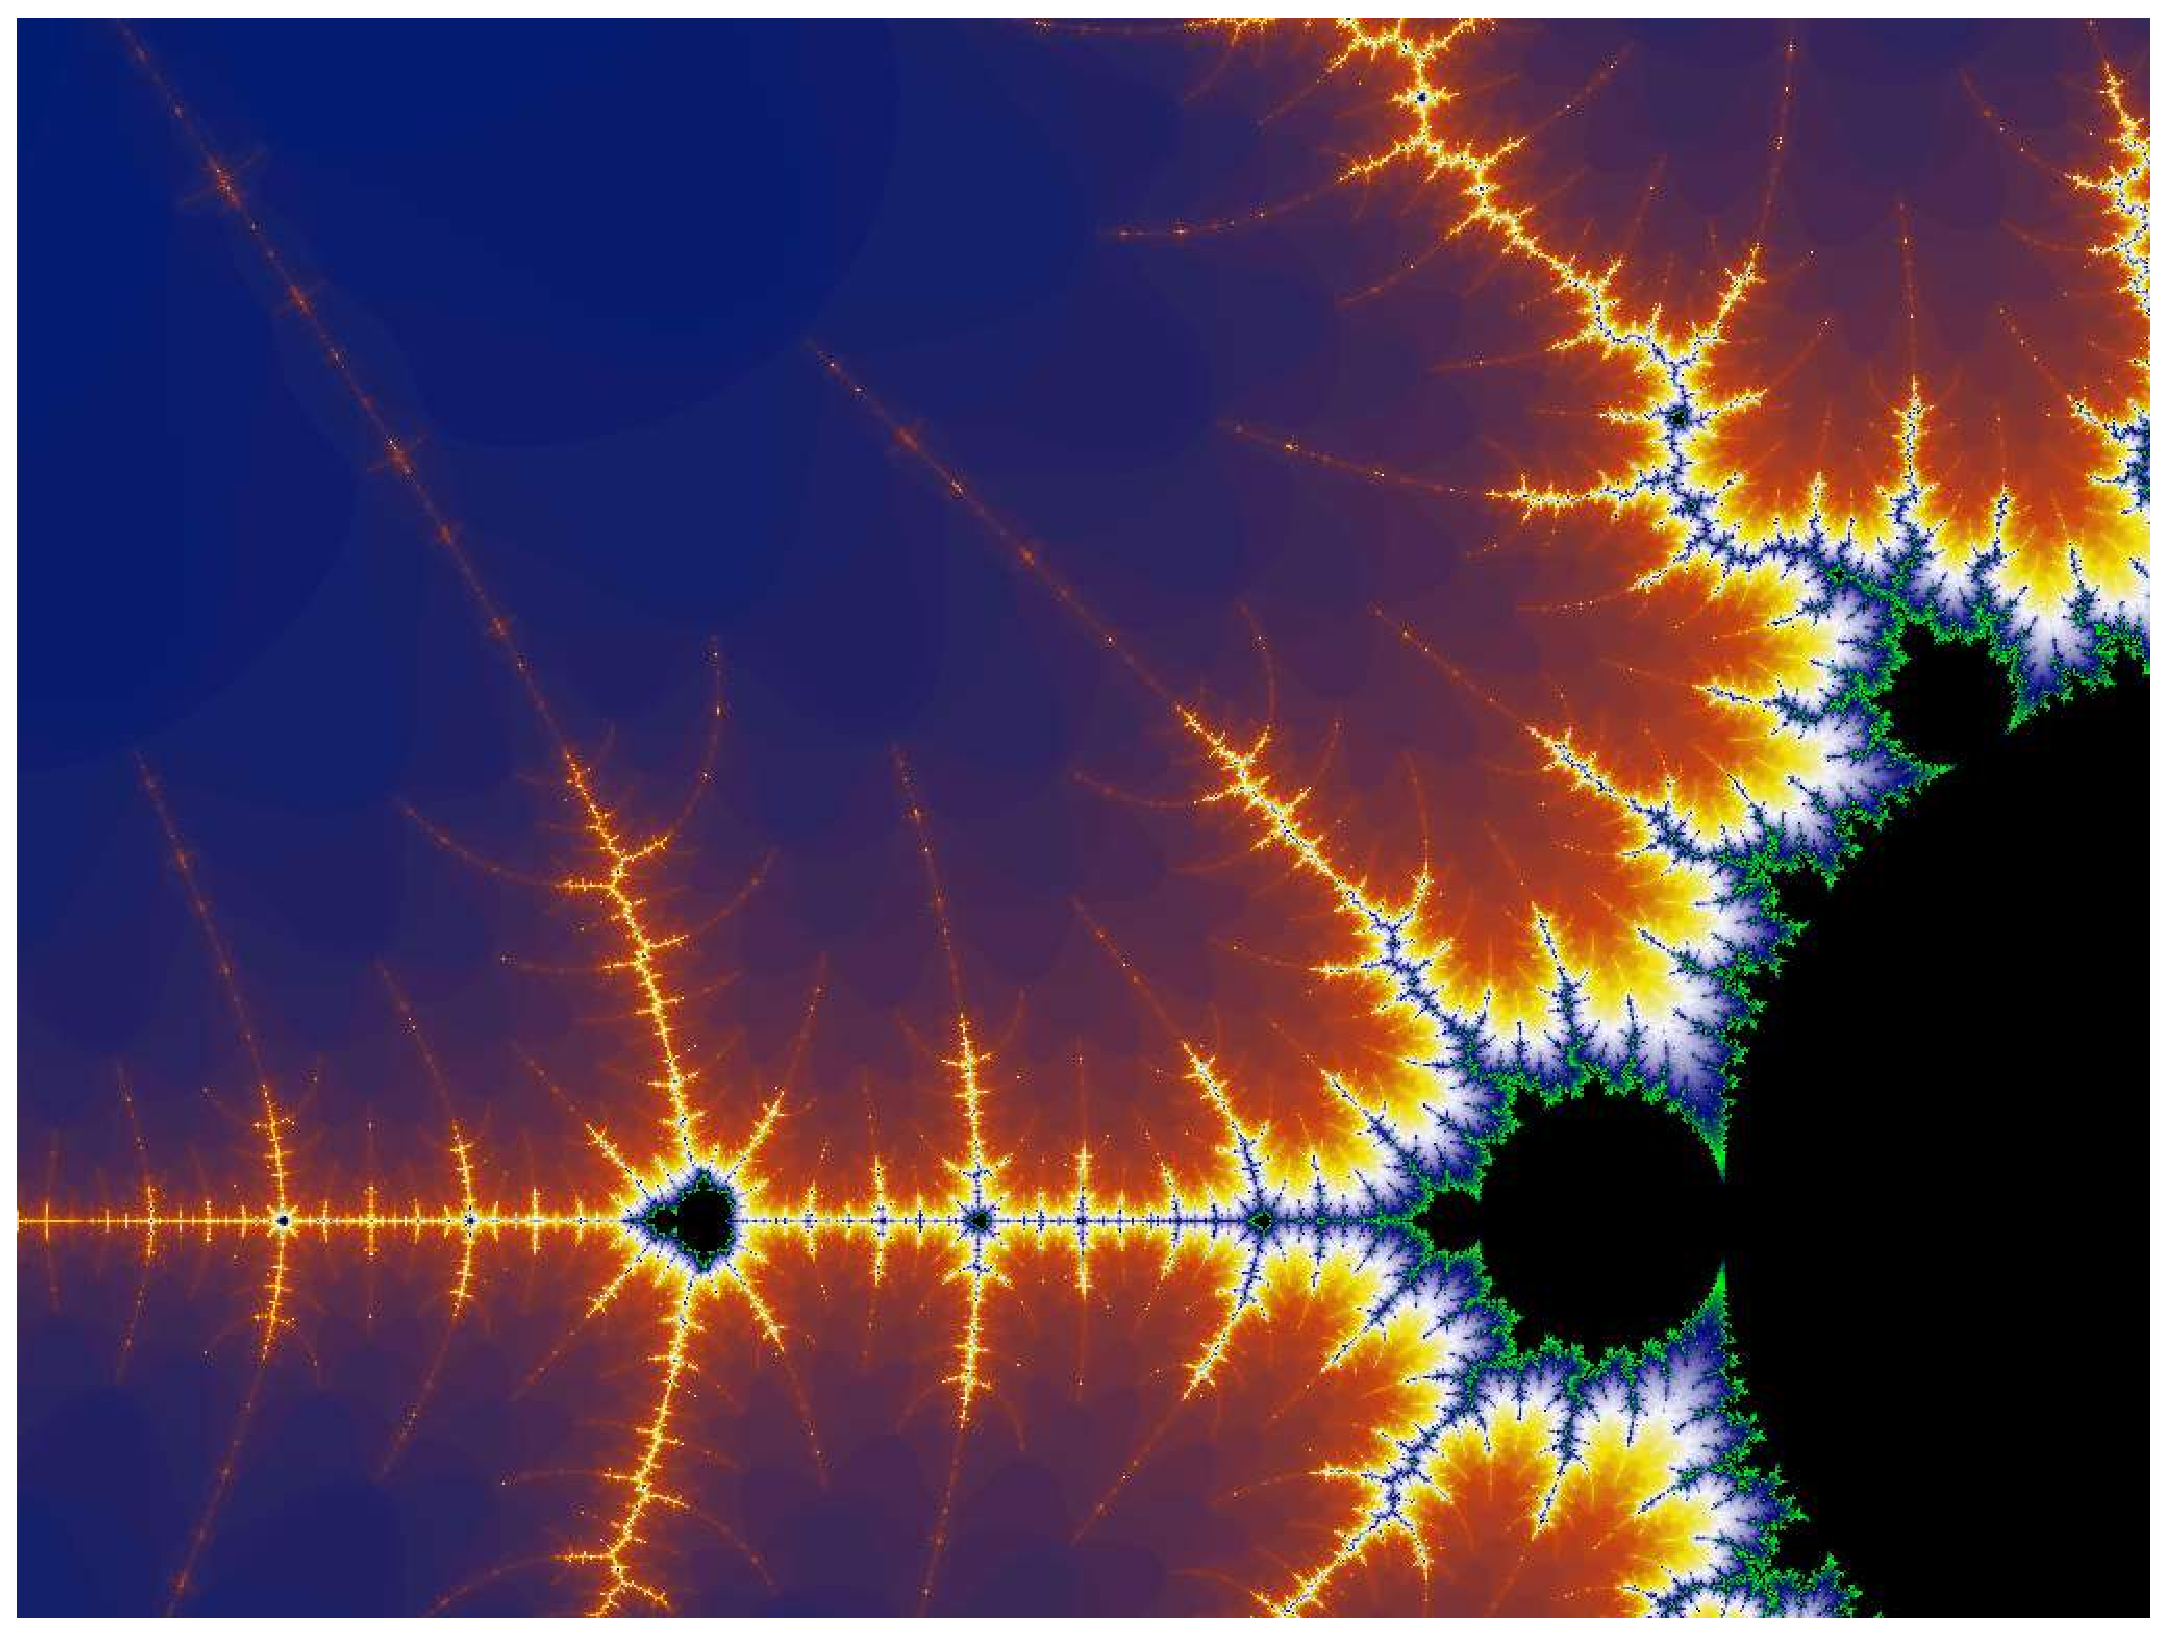
\includegraphics[scale=.2]{mandelbrot}
\caption{Mandelbrot Fractal}
\end{center}
\end{figure}
The word "fractal" often has different connotations for laypeople than mathematicians, where the layperson is more likely to be familiar with fractal art than a mathematical conception. The mathematical concept is difficult to formally define even for mathematicians, but key features can be understood with little mathematical background.

The feature of "self-similarity", for instance, is easily understood by analogy to zooming in with a lens or other device that zooms in on digital images to uncover finer, previously invisible, new structure. If this is done on fractals, however, no new detail appears; nothing changes and the same pattern repeats over and over, or for some fractals, nearly the same pattern reappears over and over. Self-similarity itself is not necessarily counter-intuitive (e.g., people have pondered self-similarity informally such as in the infinite regress in parallel mirrors or the homunculus, the little man inside the head of the little man inside the head...). 

\chapter{RELATED WORK}

The world population is the sum of all humans on Earth. As of today, it is estimated to number 7.004 billion by the United States Census Bureau. The USCB estimates that the world population exceeded 7 billion on March 12, 2012. According to a separate estimate by the United Nations Population Fund, it reached this milestone on October 31, 2011.
\begin{table}[h!]
\begin{center}
\begin{tabular}{|c|c|c|c|}
\hline Rank & Country & Population  & Percentage  \\ 
\hline 1 & China & 1,347,350,000 & 19.24\% \\ 
\hline 2 & India & 1,210,193,422  & 17.28\% \\ 
\hline 3 & United States & 313,269,000 & 4.47\% \\ 
\hline 
\end{tabular}
\caption{World Population Table} 
\end{center}
\end{table}
The world's population is unevenly distributed, with six of Earth's seven continents being permanently inhabited on a large scale. As of 2012, Asia is the most populous continent, with its 4.1 billion inhabitants accounting for over 60\% of the world population. The world's two most-populated countries alone, China and India, constitute about 37\% of the world's population. Africa is the second-most-populated continent, with around 1 billion people, or 15\% of the world's population. Europe's 733 million people make up 11\% of the world's population, while the Latin American and Caribbean regions are home to 589 million (9\%).


\chapter{DESIGN and IMPLEMENTATION}

\section{Design}
In number theory, Fermat's Last Theorem states that no three positive integers a, b, and c can satisfy the equation:
$$
a^{n} + b^{n} = c^{n}
$$ 
for any integer value of n greater than two 

This theorem was first conjectured by Pierre de Fermat in 1637, famously in the margin of a copy of Arithmetica where he claimed he had a proof that was too large to fit in the margin. No successful proof was published until 1995 despite the efforts of countless mathematicians during the 358 intervening years. The unsolved problem stimulated the development of algebraic number theory in the 19th century and the proof of the modularity theorem in the 20th. It is among the most famous theorems in the history of mathematics and prior to its 1995 proof was in the Guinness Book of World Records for "most difficult mathematical problems".

\subsection{Stirlings approximation}
In mathematics, Stirling's approximation (or Stirling's formula) is an approximation for large factorials. It is named after James Stirling.

The formula as typically used in applications is:

$$
\ln (n!) = n \ln n - n  + O(\ln(n))
$$

\section{Implementation}

Your implementation details goes here

Lorem ipsum dolor sit amet, consectetur adipiscing elit. Morbi urna mauris, sagittis sit amet aliquet ut, facilisis et nibh. Praesent turpis tortor, dignissim ut interdum eu, porttitor ut orci. Curabitur laoreet malesuada fermentum. In posuere, purus eu pulvinar luctus, eros urna tempor magna, eu tincidunt erat eros nec turpis. Vestibulum at semper lacus. Nullam tristique lacus vel nibh porta a vehicula tellus volutpat. Pellentesque cursus ullamcorper ante, ut eleifend nisl aliquam id. Nulla porta ornare fermentum. Aliquam id magna sed erat malesuada viverra. Donec non mauris eros, nec egestas ligula. Suspendisse eu tempor ligula. Aliquam egestas nulla vel augue iaculis iaculis nec in risus. Pellentesque habitant morbi tristique senectus et netus et malesuada fames ac turpis egestas. Praesent malesuada fringilla sapien a faucibus.

Lorem ipsum dolor sit amet, consectetur adipiscing elit. Morbi urna mauris, sagittis sit amet aliquet ut, facilisis et nibh. Praesent turpis tortor, dignissim ut interdum eu, porttitor ut orci. Curabitur laoreet malesuada fermentum. In posuere, purus eu pulvinar luctus, eros urna tempor magna, eu tincidunt erat eros nec turpis. Vestibulum at semper lacus. Nullam tristique lacus vel nibh porta a vehicula tellus volutpat. Pellentesque cursus ullamcorper ante, ut eleifend nisl aliquam id. Nulla porta ornare fermentum. Aliquam id magna sed erat malesuada viverra. Donec non mauris eros, nec egestas ligula. Suspendisse eu tempor ligula. Aliquam egestas nulla vel augue iaculis iaculis nec in risus. Pellentesque habitant morbi tristique senectus et netus et malesuada fames ac turpis egestas. Praesent malesuada fringilla sapien a faucibus.

\chapter{TESTING}

\chapter{RESULTS}

Compiled languages arelanguages typically processed by compilers, though theoretically any language can be compiled or interpreted. The important ones are:
\begin{itemize}
\item Ada
\item C
\item C++
\item Fortran
\item Java
\end{itemize}

\chapter{CONTRIBUTIONS}

\chapter{CONCLUSION}

An intrusion detection system (IDS) \cite{nist} is a device or software application that monitors network and/or system activities for malicious activities or policy violations and produces reports to a Management Station.


Donald Ervin Knuth \cite{knuth} is a computer scientist and Professor Emeritus at Stanford University. He is the author of the seminal multi-volume work The Art of Computer Programming. Knuth has been called the "father" of the analysis of algorithms


\begin{thebibliography}{1}
\bibitem{nist} K. Scarfone and P. Mell, ``Guide to intrusion detection and prevention systems
(idps),'' \textit{NIST Special Publication}, vol. 800, no. 2007, p. 94, 2007.
\bibitem{knuth} Wikipedia, ``Donald knuth.'' \url{http://en.wikipedia.org/wiki/Donald_Knuth}.
\end{thebibliography}

\begin{appendices}
\chapter{Sample Code}
\begin{lstlisting}[language=c++]
#include <iostream>
using namespace std;
main()
{
	cout << "Hello world \n";
	return 0;
}
\end{lstlisting}
\end{appendices}


\end{document}
